\documentclass[tikz,border=1mm]{standalone}
\usepackage{amssymb}
\usetikzlibrary{matrix,chains,positioning,decorations.pathreplacing,arrows,shapes.geometric}

% Code modified from here https://tex.stackexchange.com/questions/505741/architecture-neural-network-with-weights

\begin{document}
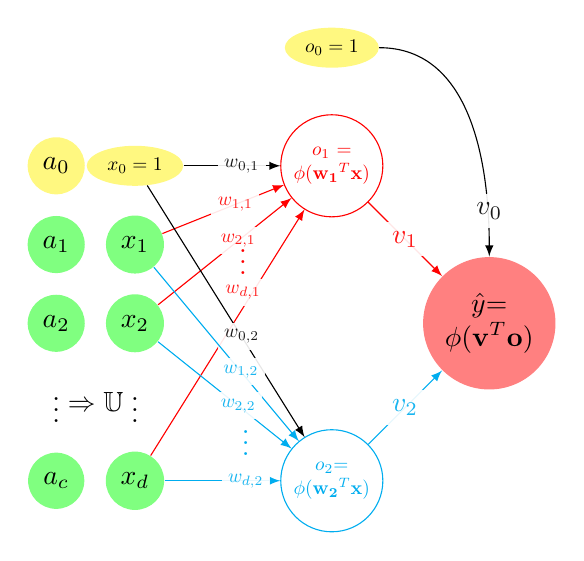
\begin{tikzpicture}[>=latex]

% Step 1 
\path
(0,1)     node[circle,draw,red, align=center, scale=0.7] (S1) {$o_1$ =\\ $\phi(\mathbf{w_1}^T\mathbf{x})$} 
+(-2.5,0) node[ellipse,fill=yellow!50, scale=0.7]  (b) {$x_0=1$}
+(-2.5,-1)  node[circle,fill=green!50]  (x1) {$x_1$}
+(-2.5,-2)    node[circle,fill=green!50]  (x2) {$x_2$}
+(-2.5,-3) node  ()  {$\vdots$}
+(-2.5,-4) node[circle,fill=green!50]  (xd) {$x_d$} 
% Input layer
+(-3.5,0)  node[circle,fill=yellow!50]  (i0) {$a_0$}
+(-3.5,-1)    node[circle,fill=green!50]  (i1) {$a_1$}
+(-3.5,-2) node[circle,fill=green!50]  (i2) {$a_2$}
+(-3.5,-3) node  ()  {$\vdots$}
+(-3.,-3) node  ()  {$\Rightarrow{\mathbb{U}}$}
+(-3.5,-4) node[circle,fill=green!50]  (ib) {$a_c$};


\draw[->, black] (b)--(S1) node[pos=.6, fill=white, opacity=.9, scale=0.7]{$w_{0,1}$};
\draw[->, red] (x1)--(S1) node[pos=.6,fill=white, opacity=.9, scale=0.7]{$w_{1,1}$};
\draw[->, red] (x2)--(S1) node[pos=.6,fill=white, opacity=.9, scale=0.7]{$w_{2,1}$}; 
\draw[->, red] (xd)--(S1) node[pos=.6,fill=white, opacity=.9, scale=0.7, above=.2mm]{$w_{d,1}$} node[pos=.6,above=3mm]{$\vdots$};
% End step 1 


% Step 2 
\path 
(0,-3)     node[circle,draw,cyan, align=center, scale=0.7] (S2) {$o_2$=\\ $\phi(\mathbf{w_2}^T\mathbf{x})$};
\draw[->, black] (b)--(S2) node[pos=.6,fill=white, opacity=.9, scale=0.7]{$w_{0,2}$};
\draw[->, cyan] (x1)--(S2) node[pos=.6,fill=white, opacity=.9, scale=0.7]{$w_{1,2}$};
\draw[->, cyan] (x2)--(S2) node[pos=.6,fill=white, opacity=.9, scale=0.7]{$w_{2,2}$}; 
\draw[->, cyan] (xd)--(S2) node[pos=.7,fill=white, opacity=.9, scale=0.7]{$w_{d,2}$} node[pos=.7,above=2mm]{$\vdots$};
% end of Step 2

% % % step 3: 
\path 
(0,2.5)  node[ellipse,fill=yellow!50, align=center, scale=0.7]  (hidden_bias) {$o_0=1$}  % bias neuron for hidden 
(2,-1)  node[circle,fill=red!50, align=center]  (y) {$\hat{y}$=\\ $\phi(\mathbf{v}^T\mathbf{o})$}; % final output neuron

% \draw[->, black] (hidden_bias)--(y) node[pos=.7,above]{$v_{0}$};
\draw [black, ->] (hidden_bias) to [out=0,in=90] (y) node[above=12mm, fill=white, opacity=.9]{$v_{0}$};
\draw[->, red] (S1)--(y) node[pos=.5,fill=white, opacity=.9]{$v_{1}$};
\draw[->, cyan] (S2)--(y) node[pos=.5,fill=white, opacity=.9]{$v_{2}$};

\end{tikzpicture}
\end{document}
